%28/10 - Fátima Sánchez Cabo
\chapter{Introducción a la genómica: caracterización del genoma mediante NGS}
\section{Introducción a la genómica traslacional}
\subsection{Definición e importancia de la genómica}
La genómica, el estudio integral del ADN y de la estructura, función y dinámica de los genomas, representa un pilar fundamental en la biología moderna. Marcó un cambio de paradigma, pasando de un enfoque reduccionista en biología - donde se estudiaban componentes individuales y de manera aislada - a una perspectiva integradora que analiza las interacciones y relaciones entre los distintos elementos biológicos. Esta transición permitió evolucionar de la genética clásica, basada en hipótesis concretas, hacia la genómica, que integra análisis de datos masivos sin necesidad de preguntas iniciales específicas, aunque sí en constante búsqueda de respuestas biológicas complejas.

En el marco del dogma central de la biología, las “ómicas” representan tres niveles de estudio: la genómica (centrada en el ADN), la transcriptómica (ARN) y la proteómica (proteínas). Este curso se enfoca en la genómica, ya que la información genética determina las funciones bioquímicas y, por ende, los fenotipos de los organismos. Gracias a avances recientes, ahora es posible inferir la función bioquímica de las proteínas directamente a partir de la secuencia de ADN, sin necesidad de técnicas complejas como la cristalización. Además, herramientas de inteligencia artificial pueden predecir la estructura de las proteínas con precisión, acelerando la interpretación de funciones biológicas.

Las proteínas, incluyendo enzimas esenciales, son los elementos funcionales clave en la biología. La secuencia de aminoácidos en una cadena polipeptídica define sus propiedades funcionales, y, por tanto, conocer la secuencia genética subyacente (el ADN) facilita predecir la función de una proteína. Aunque determinar experimentalmente las propiedades de una proteína es complejo, la secuenciación genómica ha simplificado enormemente este proceso.

La mejora en tecnologías de secuenciación impulsó el \textbf{Proyecto Genoma Humano}, que logró identificar entre 20,000 y 25,000 genes y determinar la secuencia de los aproximadamente 3 mil millones de pares de bases del genoma humano. Este proyecto también fomentó la creación de bases de datos y herramientas para el análisis de datos genómicos, además de abrir el debate sobre los aspectos éticos, legales y sociales (conocidos como ELSI, por sus siglas en inglés), que siguen siendo temas vigentes y complejos en la actualidad.

\paragraph{Evolución de la bioinformática en la genómica}
La bioinformática ha crecido a la par de la genómica en múltiples niveles. Inicialmente, era una \textbf{disciplina} incipiente y se desarrollaba como apoyo experimental; sin embargo, ha evolucionado hasta convertirse en un campo esencial que impulsa la investigación. En cuanto a su \textbf{material, los datos,} la bioinformática ha tenido que adaptarse al fenómeno del big data, pasando de manejar cantidades limitadas de datos a enfrentar volúmenes masivos, propios de la genómica actual. Paralelamente, el \textbf{rol de los bioinformáticos} se transformó, pasando de ser técnicos a científicos de datos y académicos altamente reconocidos en la industria y en la investigación.

\begin{figure}[htbp]
\centering
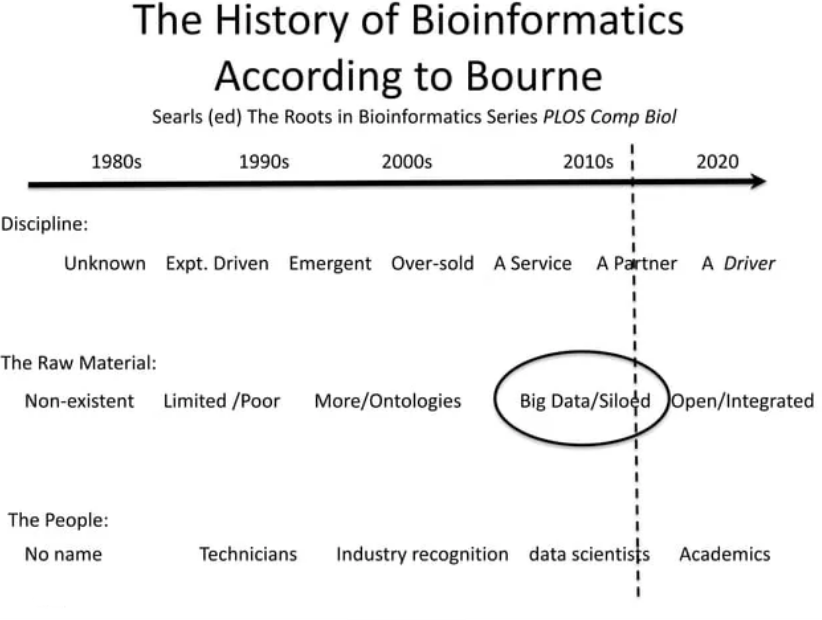
\includegraphics[width = 0.5\textwidth]{figs/history-bioinfo.png}
\caption{Breve historia de la bioinformática en tres niveles: como disciolina, como material que utiliza y como las personas que trabajan en ella. Evolución desde 1980 hasta 2020.}
\end{figure}

\subsection{Avances tecnológicos en secuenciación}
Existen distintos tipos de tecnologías de secuenciación, comúnmente clasificadas en tres generaciones: la primera generación (first generation), la segunda o Next Generation Sequencing (NGS) y la tercera generación. Las dos primeras generaciones se enfocan en la secuenciación de fragmentos cortos de ADN, mientras que la tercera generación permite la lectura de fragmentos largos, facilitando el ensamblaje completo de genomas. Actualmente, uno de los mayores desafíos tecnológicos es detectar variantes de baja frecuencia y realizar secuenciaciones de ADN en células individuales (single-cell sequencing), lo cual tradicionalmente se hacía de forma masiva (“bulk”).

\begin{figure}[htbp]
\centering
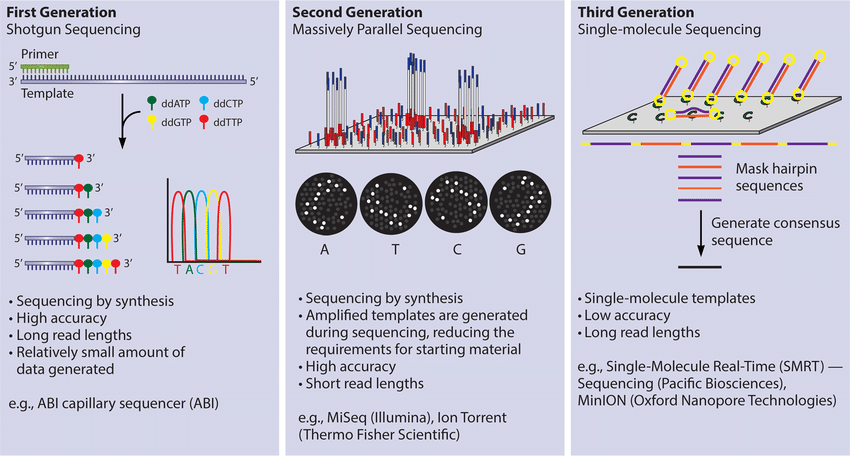
\includegraphics[width = 0.7\textwidth]{figs/sequencing-generations.png}
\caption{Las tres generaciones de secuenciación y su forma de actuar.}
\end{figure}

A medida que el costo de la secuenciación ha disminuido y la capacidad de almacenamiento ha mejorado desde 1990, los datos generados también han crecido exponencialmente. En un experimento de secuenciación, los costos abarcan tanto la secuenciación en sí como el procesamiento bioinformático, el reporte y el almacenamiento de los datos. La comunidad científica y muchos journals requieren que los datos de proyectos financiados públicamente estén disponibles en bases de datos accesibles, lo que asegura la transparencia y el acceso a esta información valiosa. Para obtener una cobertura de calidad, el ADN suele secuenciarse al menos 30 veces, lo que genera archivos de gran tamaño, como los archivos FastQ, que almacenan información de secuencia y calidad para cada base.

\subsection{Procesos de llamada y priorización de variantes}
Los datos de secuenciación se procesan en pipelines bioinformáticas que comienzan con archivos FastQ normalmente comprimidos y pasan por varias etapas: control de calidad, alineamiento y llamada de variantes (variant calling). Las variantes identificadas pueden incluir cambios de nucleótidos, variaciones en el número de copias de segmentos genómicos (copy number variation) o reordenamientos estructurales.

\begin{figure}[htbp]
\centering
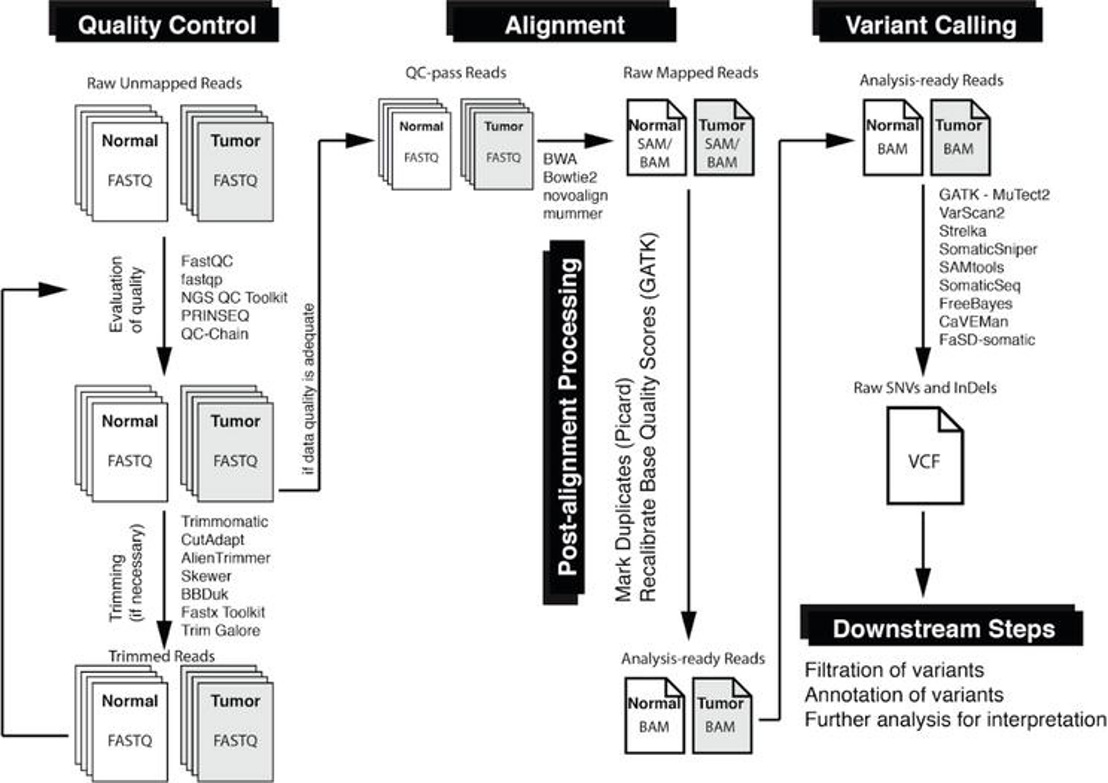
\includegraphics[width = 0.7\textwidth]{figs/bioinfo-pipeline.png}
\caption{Esquema de la pipeline que se sigue en bioinformática para la llamada de variantes.}
\end{figure}

La priorización de variantes se basa en factores como el impacto funcional, la frecuencia alélica en la población y la asociación con enfermedades. Sin embargo, muchas variantes requieren validación experimental, frecuentemente en modelos animales como ratones, para corroborar su relevancia funcional. El proceso de filtrado inicial se enfoca en variantes en exones de genes candidatos, analizando su frecuencia, patogenicidad y modelo de herencia; en caso de no hallarse variantes relevantes, se amplía el análisis a variantes oligogénicas o no codificantes.

\begin{figure}[htbp]
\centering
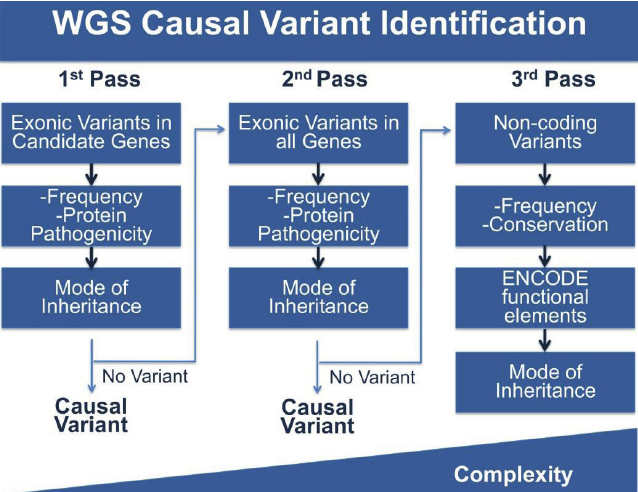
\includegraphics[width = 0.5\textwidth]{figs/variant-priorization.png}
\caption{Ejemplo de la priorización de variantes.}
\end{figure}

\subsection{Genómica en medicina de precisión}
La genómica ha transformado el enfoque de la medicina de precisión, permitiendo identificar enfermedades con bases genéticas, ambientales o una combinación de ambas. Algunas variantes genéticas confieren una predisposición a enfermedades sin ser causantes directas, lo cual es crucial para inferir relaciones causales y acelerar ensayos clínicos mediante la integración de grandes volúmenes de datos. Estas variantes pueden clasificarse en germinales (heredadas) o somáticas (adquiridas).

\begin{figure}[htbp]
\centering
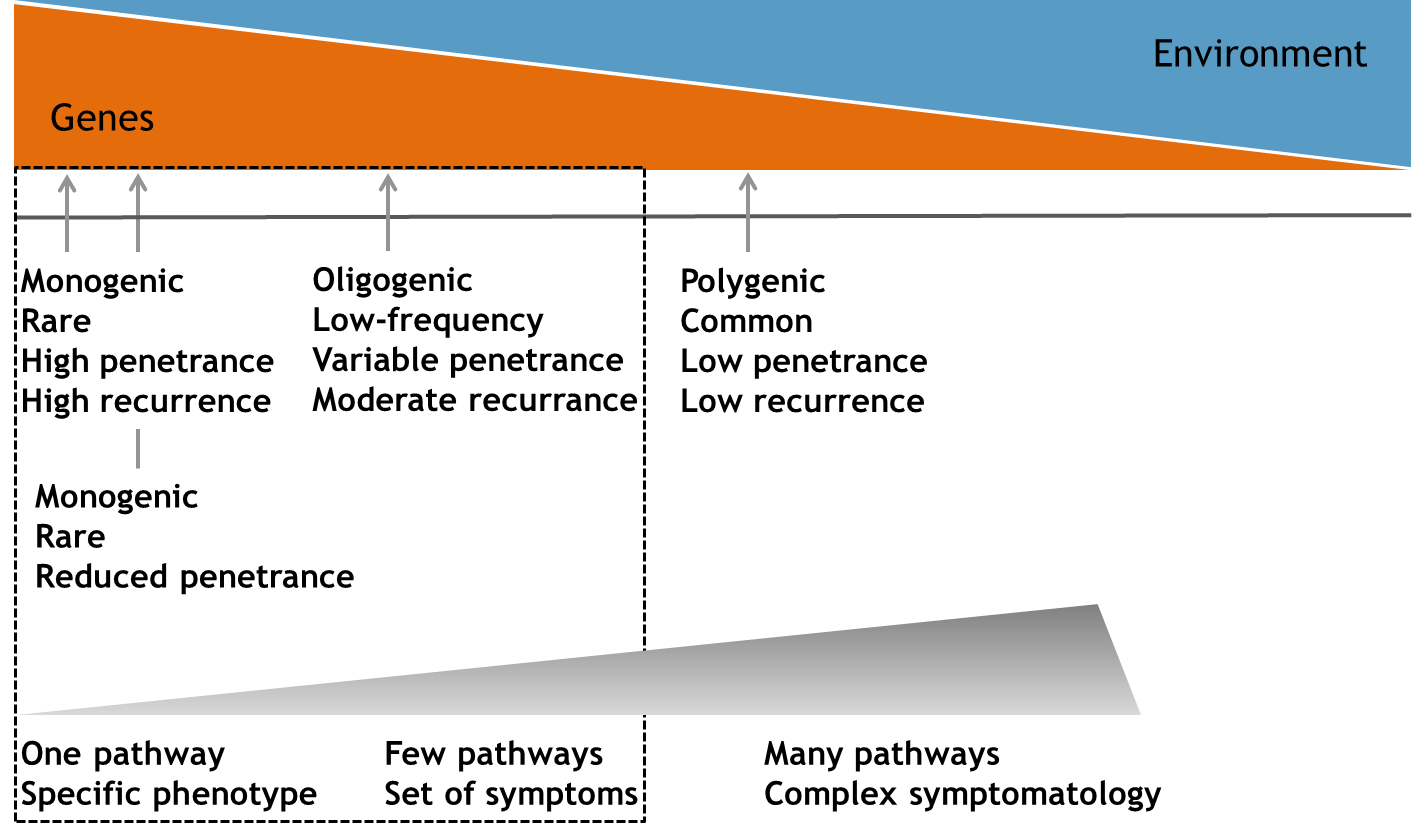
\includegraphics[width = 0.5\textwidth]{figs/genetic-environment.png}
\caption{Representación gráfica de la relación entre enfermedades con base genética, ambientales o una mezcla de ambas.}
\end{figure}

En medicina de precisión, la genómica es solo una capa de datos entre muchas. Para una comprensión holística de la salud y la enfermedad, es necesario combinarla con información de otras “ómicas” como la transcriptómica, epigenómica, proteómica, metabolómica, y datos de microbioma. Además, los datos clínicos y epidemiológicos también forman parte del ecosistema de \textbf{Big Data Biomédico}, que actualmente se maneja mediante técnicas avanzadas de computación en clusters HPC, computación en la nube y algoritmos de GPU.

\begin{figure}[htbp]
\centering
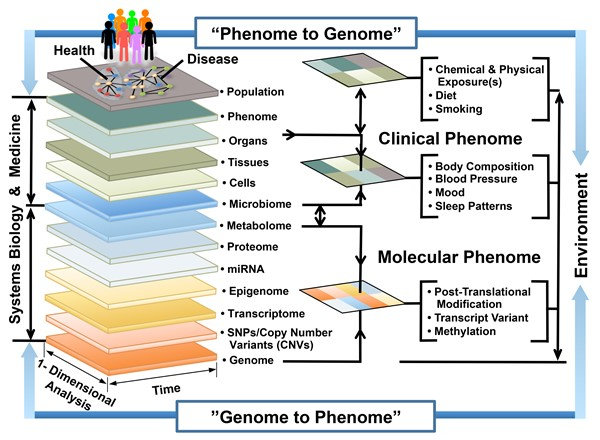
\includegraphics[width = 0.7\textwidth]{figs/bigger-picture-bioinfo.jpg}
\caption{Esquema representando el dibujo general de la bioinformática.}
\end{figure}

Varias bases de datos públicas permiten estudiar la transición entre salud y enfermedad. El estudio de Farmingham, por ejemplo, lleva más de 70 años recolectando datos de factores de riesgo cardiovascular en más de 15,000 participantes. En Reino Unido, el Biobank y, en Estados Unidos, la iniciativa All of Us, también representan recursos de gran envergadura. En España, el CNIC (Centro Nacional de Investigaciones Cardiovasculares) realiza el estudio PESA (Progression of Early Subclinical Atherosclerosis), que ha contribuido a identificar factores predictivos de aterosclerosis subclínica mediante el estudio multiómico, generando nuevos indicadores con un mayor poder predictivo de la formación de placas de colesterol.

\paragraph{Epigenética y la medición de la edad biológica}
El perfil de metilación del ADN es un factor epigenético que puede modificar la expresión genética y se ha utilizado para calcular la “edad biológica” o epigenética de una persona, lo que puede servir como predictor de esperanza de vida y salud. Al comparar estos perfiles con la edad cronológica, sexo y otros factores, se obtiene información sobre el envejecimiento y el riesgo de enfermedades, facilitando el desarrollo de estrategias de salud personalizadas.

\subsection{Resumen}
La genómica ha liderado una revolución científica en el siglo XX, evolucionando desde el estudio de componentes individuales hasta una perspectiva integral de sistemas biológicos y de investigación basada en datos masivos. La bioinformática se ha convertido en una disciplina central en el análisis genómico y predicción de estructuras proteicas, impulsada por el Proyecto Genoma Humano y el desarrollo de tecnologías de secuenciación. Los avances actuales buscan no solo la secuenciación del ADN, sino también la integración de estos datos con datos epidemiológicos y moleculares para obtener una comprensión más profunda de la salud y la enfermedad. Así, el Proyecto Genoma Humano fue decisivo para sentar las bases de tecnologías de secuenciación, el desarrollo de la bioinformática en sí y el uso social e industrial de los datos ómicos.

La identificación de características genómicas relevantes causales de rasgos/enfermedades se basa en la anotación de variantes en bases de datos y en estudios poblacionales: hay margen de mejora y un gran éxito de la ciencia colaborativa. Hoy en día, los principales proyectos tratan no sólo de secuenciar el ADN, sino de integrar esta información con datos epidemiológicos y otros datos moleculares para comprender mejor la salud y la enfermedad.
Las enfermedades, en función de su base genética, pueden clasificarse en monogénicas (mendelianas), oligogénicas (ej., cardiopatías familiares) y complejas (evaluadas mediante puntuaciones de riesgo poligénicas). Esta clasificación permite avanzar en la medicina de precisión, abordando enfermedades desde su origen genético para ofrecer intervenciones de salud más efectivas y personalizadas.

%30/10 - Álvaro Serrano
\section{Métodos de secuenciación}
La secuenciación permite pasar de la información contenida en el ADN a un dominio digital mediante una representación abstracta. 

El primer método de secuenciación fue el \textbf{método Maxam-Gilbert}, que utilizaba un marcador en el extremo 5' del ADN. En este proceso, el ADN se trataba con diferentes compuestos químicos para provocar rupturas específicas en función de cada base nitrogenada. Los fragmentos resultantes se separaban en un gel de acrilamida mediante electroforesis, y se revelaban mediante autoradiografía de rayos X. La secuencia se deducía observando el patrón de bandas resultante.

\begin{figure}[htbp]
\centering
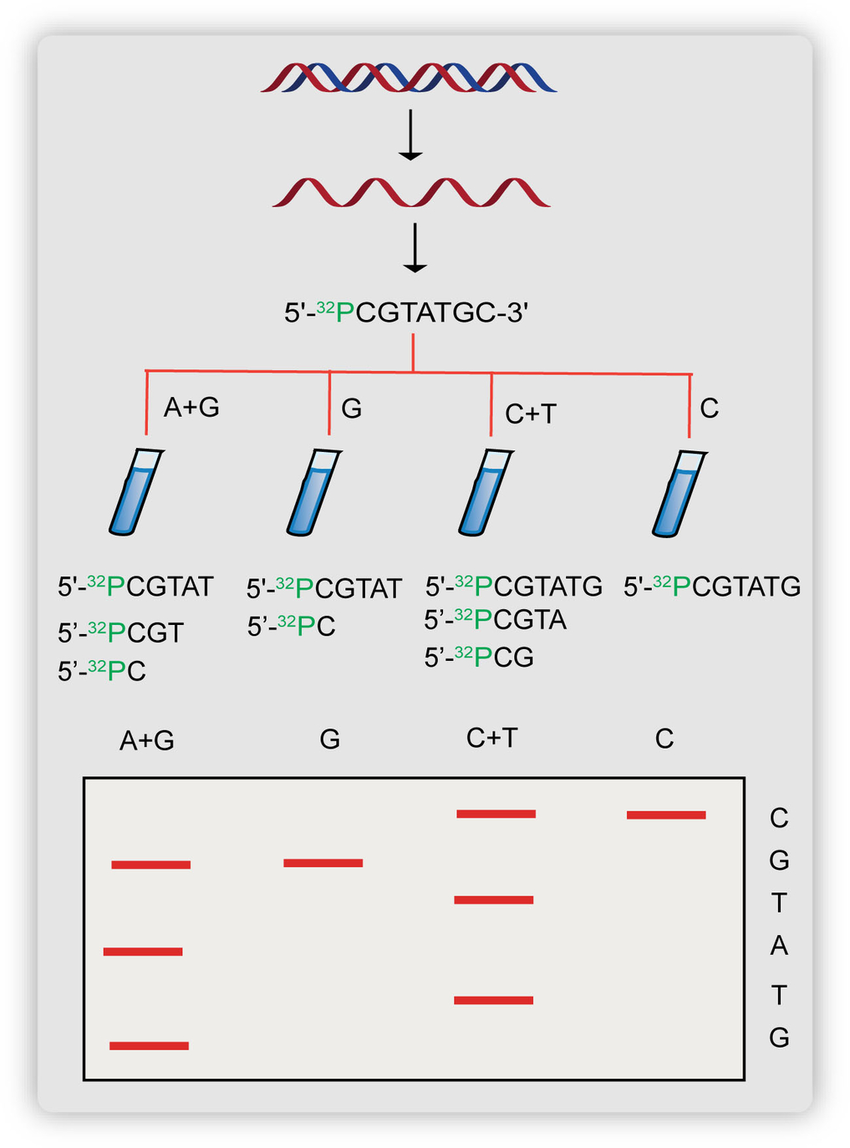
\includegraphics[width = 0.3\textwidth]{figs/maxam-gilbert.png}
\caption{\textbf{Principio de la secuenciación Maxam-Gilbert}: Se llevaron a cabo cuatro reacciones separadas para la degradación de bases en un fragmento de ADN monocatenario: A+G, G, C+T y C. Se obtienen fragmentos de ADN de diferente longitud tras la degradación de las bases y la escisión del esqueleto de azúcar-fosfato. Los productos se cargan en cuatro pocillos separados de un gel de poliacrilamida. La secuencia se lee de abajo a arriba como GTATGC. Si se encuentra una G frente a un hueco en el gel, se confirma que se trata de 5-metilcitosina en la cadena molde.}
\end{figure}

Otro método clave es el de \textbf{terminación de cadena, o método de Sanger}. Este utiliza deoxinucleótidos modificados, que tienen un átomo de hidrógeno en el grupo 2' de la pentosa, en lugar de un grupo hidroxilo (OH). Esto impide la unión del extremo 5' al 3', deteniendo así la extensión de la cadena de ADN. El resultado es una mezcla de fragmentos de distintos tamaños, los cuales se marcan con isótopos radioactivos o, en versiones más modernas, con fluoróforos. La secuencia se obtiene mediante detección de colores en una única reacción, simplificando el análisis. La clave de este método \marginpar[\footnotesize Pregunta examen] \ es el uso de dideoxinucleótidos, que interrumpen la actividad de la ADN polimerasa, permitiendo detener la cadena de manera controlada.

\begin{figure}[htbp]
\centering
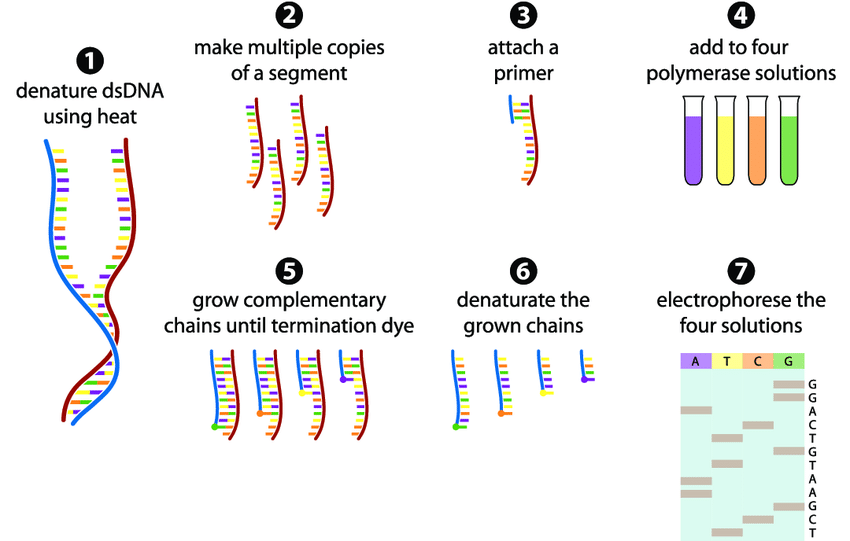
\includegraphics[width = 0.8\textwidth]{figs/sanger.png}
\caption{\textbf{El método de secuenciación Sanger en 7 pasos.} (1) El fragmento de dsADN se desnaturaliza en dos fragmentos de ssADN. (2) Un fragmento de ssADN se multiplica en millones de copias. (3) Se une un cebador que corresponde a un extremo del fragmento. (4) Los fragmentos se añaden a cuatro soluciones de polimerasa. Cada solución contiene los cuatro tipos de bases pero sólo un tipo de nucleótido de terminación. (5) La cadena crece hasta que se añade aleatoriamente un nucleótido de terminación. (6) Los fragmentos de dsADN resultantes se desnaturalizan para obtener una serie de ssADN de distintas longitudes. (7) Los fragmentos se separan por electroforesis y se lee la secuencia.}
\end{figure}

El primer secuenciador automático fue el ABI370, capaz de secuenciar hasta 5000 bases al día. Sin embargo, se necesitarían aproximadamente 16,000 años para secuenciar todo el genoma humano usando esta tecnología. Este secuenciador innovador reemplazaba los geles por electroforesis capilar y un detector de fluorescencia. Durante el Proyecto Genoma Humano en los años 90 y 2000, desarrollado en colaboración entre el sector público y privado, se introdujeron mejoras significativas a los secuenciadores, como el modelo ABI377, que empleaba varios capilares para incrementar la eficiencia. Sin embargo, la secuenciación de regiones altamente repetitivas del genoma, como los telómeros y centrómeros, fue compleja, y la primera descripción completa del genoma humano fue publicada hace apenas un año.

\subsection{Métodos de secuenciación empleados en el Proyecto Genoma Humano}
Los métodos que se utilizaron en el proyecto fueron los siguientes:
\begin{itemize}
\item \textbf{Hierarchical Shotgun:} En este método, el ADN se clona en fragmentos más pequeños usando enzimas de restricción. Estos fragmentos se solapan y forman contigs, los cuales se ensamblan progresivamente para reconstruir la secuencia original.
\item \textbf{Whole-genome Shotgun:} Similar al método anterior, pero se realiza directamente sobre el genoma completo en lugar de partir de cromosomas bacterianos. El ADN se clona en bacterias, se fragmenta y se ensamblan los contigs mediante solapamiento.
\end{itemize}

\begin{figure}[htbp]
\centering
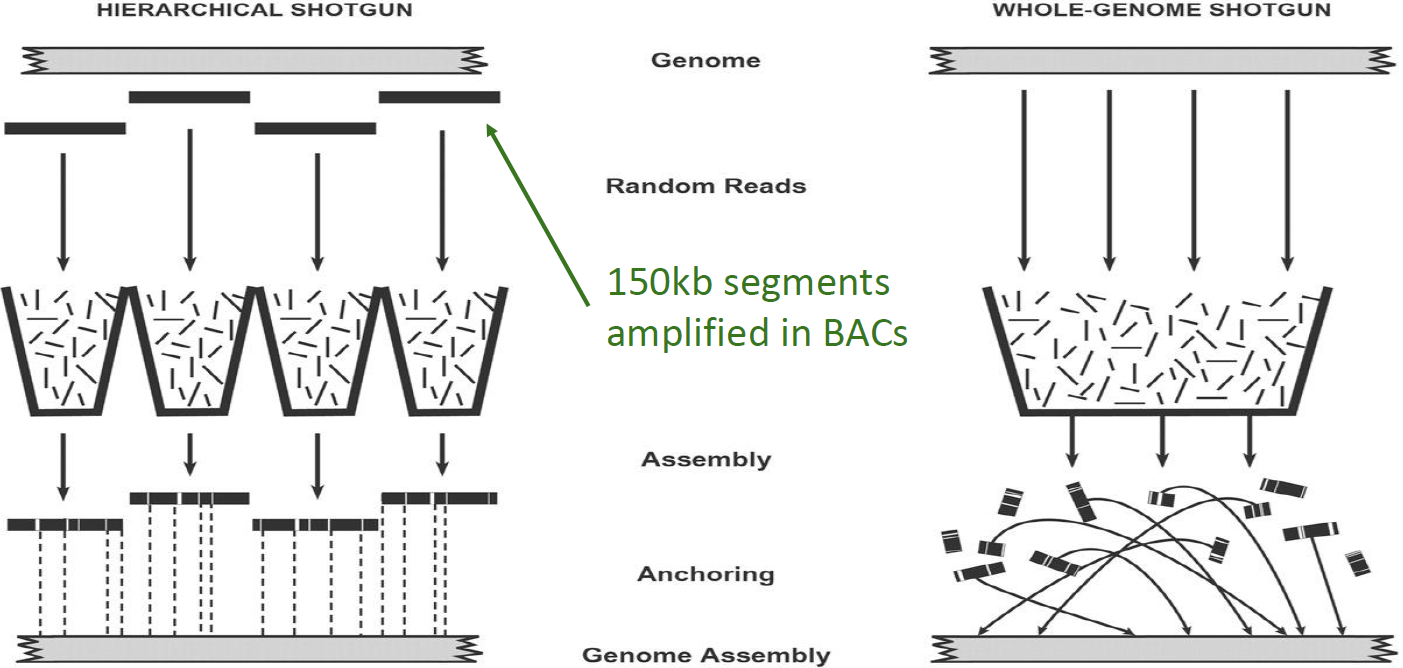
\includegraphics[width = 0.8\textwidth]{figs/HGP-sequencing.png}
\caption{\textbf{Estrategias de secuenciación en el Proyecto Genoma Humano.} (Izquierda) La estrategia de hierarchical shotgun (HS) consiste en descomponer el genoma en un camino de mosaico de clones BAC (bacterial artificial chromosome) superpuestos, realizar la secuenciación en cada BAC y volver a ensamblarlo, y luego fusionar las secuencias de clones adyacentes. El método tiene la ventaja de que todos los contigs de secuencias y scaffolds derivados de un BAC pertenecen a un único compartimento con respecto al anclaje al genoma. (Derecha) La estrategia WGS (Whole-genome shotgun) consiste en secuenciar todo el genoma e intentar reensamblar toda la colección. Con el método WGS, cada contig y scaffold es un componente independiente que debe anclarse al genoma. En general, muchos scaffolds no pueden anclarse sin esfuerzos dirigidos. (Los contigs son bloques contiguos de secuencia; los scaffolds son conjuntos de contigs unidos por lecturas emparejadas de ambos extremos de un inserto plasmídico).}
\end{figure}

La electroforesis capilar, usada en ambos métodos, permite separar fragmentos de ADN de diferentes tamaños a través de un capilar con un detector de fluorescencia, logrando una lectura precisa de aproximadamente 500 pares de bases por fragmento. Con el tiempo, los costos de secuenciación disminuyeron gracias a avances en técnicas posteriores al método de Sanger.

\subsection{NGS: la siguiente generación de tecnología de secuenciación del ADN}
La secuenciación de segunda generación o Next-Generation Sequencing (NGS) permite una secuenciación paralela y masiva, también conocida como \textbf{high-throughput sequencing}. Los principales métodos NGS incluyen 454 Roche, Solexa Illumina, ABI/SOLiD, Complete Genomics, Pacific Biosciences, Ion Torrent y Oxford Nanopore.

\subsubsection{Preparación de librerías de NGS}
Las librerías de secuenciación se preparan fragmentando el ADN y generando secuencias que luego se amplifican y procesan en el secuenciador, obteniendo las lecturas o reads. Estas librerías se amplifican clonalmente mediante tres métodos:
\begin{itemize}
\item \textbf{Beads:} pequeñas bolitas recubiertas de primers, donde el ADN se adhiere y se amplifica.
\item \textbf{Fase sólida:} el ADN se adhiere a una superficie de cristal donde se amplifica.
\item \textbf{Nanobolas:} se produce un ovillo de ADN amplificado en forma circular, que se adhiere a una placa metálica funcionalizada (con grupos funcionales) para secuenciación.
\end{itemize}

La secuenciación NGS utiliza un gran número de moléculas idénticas, permitiendo una secuenciación paralela de alta eficiencia y alto rendimiento o high-throughput. La característica de la segunda generación es que utiliza la molécula de ADN original y, sobre ella, la amplifica, es decir, la utiliza como molde para generar muchas moléculas iguales. 

\subsubsection{Clasificación de NGS: secuenciación por síntesis y por ligación}
Los métodos de secuenciación de segunda generación se pueden clasificar en secuenciación por síntesis (con la enzima polimerasa) o secuenciación por ligación (con la enzima ligasa).

\begin{itemize}
\item \textbf{Secuenciación por síntesis (SBS)}
\begin{itemize}
\item \textbf{Ciclo de terminación reversible (CRT):} una evolución del método Sanger. Se utiliza ADN unido a beads o cristales y se añaden dNTPs modificados con el grupo 3’ OH bloqueado, limitando así la duplicación de la polimerasa. Cada ciclo implica la incorporación de un nucleótido, seguido de una señal fluorescente específica del nucleótido unido. Posteriormente, el grupo OH se desbloquea con un químico de lavado para que el proceso continúe. La señal que se detecta no es de un único nucleótido, si no del conjunto de nucleótidos del cluster, que debido a la amplificación clonal, debería ser la misma señal amplificada. Esto se realiza por el límite de detección de fluorescencia de los microscopios. Además, la placa con los moldes tiene en los límites unos marcadores que permiten que el microscopio se enfoque a la altura a la que debe. 

Una vez terminada la secuenciación, se utiliza como primer para secuenciar la cadena contraria. Esto se debe a que el microscopio va enfocando peor y se pierde calidad. Cada señal emitida por el fluoróforo se conoce como call o llamada. Cada call tiene una confident score de Q, que se calcula mediante la fórmula $Q = - 10 log_{10} P $. Por tanto, si Q es 30, P sería $10^{-3}$, representando P la probabilidad de error. La información que se obtiene en el archivo es la secuencia obtenida con un valor Q asociado codificado en ASCII. 

Los microscopios se clasifican en microscopios de 4 canales y de 2 canales. Los microscopios de 4 canales tienen una mayor calidad al poder distinguir cada uno de los nucleótidos, mientras que los de 2 canales utilizan la combinación de dos fluoróforos: se detecta verde, rojo, la combinación entre verde y rojo, y la ausencia de fluorescencia. Esto último es algo arriesgado, ya que algunos nucleótidos podrían perder el fluoróforo y se consideraría ausencia de fluorescencia. No obstante, estos microscopios de 2 canales, pese a tener una peor calidad, son más rápidos y baratos. Respecto al secuenciador, hay varios tipos, por lo que al elegir uno se tendrá que tener cuenta el caso de uso y el dinero disponible (la página de Illumina tiene tablas comparativas para elegir el mejor secuenciador para cada caso). 

Las ventajas de la secuenciación CRT es que es la que produce la mayor cantidad de secuencias secuenciadas a la vez (mayor throughput). La desventaja es el límite que puede secuenciar, que es en torno a 150 bases por cada extremo. 

\item \textbf{Adición de nucleótidos simple (SNA):} en cada ciclo se añade un solo tipo de nucleótido, detectando su incorporación. Este método es sensible a los homopolímeros (repeticiones del mismo nucleótido), lo que puede generar problemas de fase si la señal no es proporcional al número de nucleótidos añadidos.
\begin{itemize}
\item \textbf{Pirosecuenciación:} emplea pirofosfato liberado en la síntesis de ADN. Debido a su enlace de alta energía, la acción de la pirofosfatasa acoplada a la luciferasa produce que se emita una señal de luz proporcional al número de nucleótidos añadidos. Este método es rápido, económico y preciso, aunque presenta limitaciones con secuencias largas debido al cambio de fase en el momento en el que se produzca un error. La calidad de la secuenciación es Q45 (99,997\%). 

\item \textbf{Ion Torrent proton detection:} mide el cambio de pH (cambio de potencial) que ocurre al liberar un protón durante la polimerización del ADN. Al final de cada ciclo es necesario lavar para evitar la señal cruzada. La técnica es económica y ampliamente utilizada en hospitales, pero presenta desafíos con secuencias largas debido a la falta de proporcionalidad en la señal en secuencias con regiones muy repetitivas (si se unen dos nucleótidos en lugar de uno, la señal es proporcional a los dos, pero cuando se unen 50 nucleótidos, el cambio de potencial no es proporcional a los 50).

\end{itemize}
\end{itemize}

\item \textbf{Secuenciación por ligación (SBL)}
\begin{itemize}
\item \textbf{Secuenciación por SOLiD:} Este método emplea sondas de ligación con dos bases complementarias a la base que se secuencia. En cada ciclo, una ligasa une una sonda marcada con un fluoróforo y luego se elimina la fluorescencia para repetir el ciclo, generando datos precisos, aunque menos comunes en la práctica. Se van mapeando dos nucleótidos a la vez, dejando un espacio de 3 nucleótidos. Por ello, se repite cinco veces añadiendo espaciadores que permitan el solapamiento de las lecturas.

\item \textbf{Complete Genomics (Nanoballs, BGI):} Amplifica ADN mediante rolling circle para formar ovillos, que luego se hibridan en una placa. Las sondas fluorescentes hibridan de forma iterativa para secuenciar el ADN. Este método permite una alta densidad de secuencias pequeñas, teniendo así una precisión muy alta. No obstante, permite secuenciar lecturas pequeñas y, al final, se utilizan distintos adaptadores a los que se unen las sondas, permitiendo aumentar el througput. Hay partes de la tecnología que no se conocen y está principalmente disponible en China.
\end{itemize}
\end{itemize}

%Importante a quedar claro: diferencia entre secuenciación por síntesis y por ligación, y dentro de ellos la diferencia entre el método CRT y SNA. Los métodos de ligación hay que saber que existen, pero no es habitual trabajar con ellos. 

\subsubsection{Limitaciones y desafíos en NGS}
La NGS de segunda generación presenta una tasa de error de Q25-Q35 y ciertas limitaciones:
\begin{itemize}
\item \textbf{Lecturas cortas} generan dificultades en el ensamblaje de genomas completos y en la identificación de variantes estructurales.
\item \textbf{Errores de secuenciación} especialmente en regiones complejas y repetitivas, como secuencias AT/GC (SBS) y homopolímeros (SNA).
\item \textbf{Sesgo de amplificación} algunas regiones se amplifican mejor que otras, afectando la uniformidad en las lecturas.
\item \textbf{Alto coste de los equipos}
\item \textbf{Fenómeno de la cadena retrasada} cuando no se incorpora un nucleótido, produciendo un descabalgamiento del ciclo de lectura real y el ciclo de lectura en el que creemos que estamos.
\item \textbf{Persistencia de errores en los cluster} al producirse un error en el cluster, el error se queda a lo largo de la secuenciación.
\item \textbf{Cambios epigenéticos}
\end{itemize}

%Take-home messages